\documentclass[a4paper,12pt]{article}
\usepackage{graphicx}
\usepackage{hyperref}
\usepackage{amsmath}
\usepackage{times}
\usepackage{xcolor}
\usepackage{amsfonts}
\usepackage{garamondx}
\usepackage{framed}  %This is to use the shaded environment

\usepackage{titlesec}

\titlespacing*{\section}
{0pt}{5.5ex plus 1ex minus .2ex}{4.3ex plus .2ex}
\titlespacing*{\subsection}
{0pt}{5.5ex plus 1ex minus .2ex}{4.3ex plus .2ex}

\usepackage{titling}
\setlength{\droptitle}{-8em} 


\textwidth=6.2in
\textheight=8.5in
%\parskip=.3cm
\oddsidemargin=.1in
\evensidemargin=.1in
\headheight=-.3in
\setlength{\parindent}{0pt}



% \renewcommand{\baselinestretch}{1} 
% \setlength{\parskip}{\baselineskip}
% \setlength{\parindent}{0pt}
% \setlength{\marginparwidth}{2.5cm}


\newcommand{\scscst}{\scriptscriptstyle}
\newcommand{\scst}{\scriptstyle}
\newcommand{\Robject}[1]{{\code{#1}}}
\newcommand{\Rfunction}[1]{{\code{#1}}}
\newcommand{\Rclass}[1]{\textit{#1}}
\newcommand{\Rpackage}[1]{\textit{#1}}
\newcommand{\Rexpression}[1]{\code{#1}}
\newcommand{\Rmethod}[1]{{\code{#1}}}
\newcommand{\Rfunarg}[1]{{\code{#1}}}

\newcommand\boldblue[1]{\textcolor{blue}{\textbf{#1}}}
\newcommand\code[1]{\textcolor{red}{\texttt{#1}}}

\usepackage{Sweave}
\begin{document}
\definecolor{shadecolor}{gray}{0.95} %this is defining the color of the background in the shaded environment

\Sconcordance{concordance:3_Course_Notes-knitr.tex:3_Course_Notes-knitr.Rnw:%
1 50 1 1 0 4 1 1 7 12 1 1 7 1 1 1 7 94 1 1 2 1 0 3 1 3 0 1 2 6 1 1 2 1 %
0 1 1 1 2 1 1 3 0 1 2 9 1 1 2 4 0 1 2 4 1 1 2 1 0 1 1 3 0 1 2 45 1 1 4 %
6 0 1 2 12 1 1 2 4 0 1 2 5 1}




%------------------------------------------------------------
\title{Using R as a Research Tool.}
%------------------------------------------------------------
\author{Susan Johnston: \href{mailto:Susan.Johnston@ed.ac.uk}{Susan.Johnston@ed.ac.uk}  \\ \\
        Demonstrators: Gergana Dalaskova, John Godlee. \\
        Hat-Tips to Kyle Dexter and The Coding Club.}
%\date{}









\maketitle

%\tableofcontents


%-------------------------------------------
\section {Introduction}
%--------------------------------------------

\subsection {What is \boldblue{R}?}

\boldblue{R} began its life in New Zealand in 1993 as a language and environment for statistical computing and graphics. It is an interpreted programming language, meaning that rather than pointing and clicking, the user types in commands. It is \textbf{free} and works across all platforms.


\subsection {Why use \boldblue{R}?}

\begin{center}
``\texttt{This is R. There is no if. Only how.}'' \\
\texttt{{-}{-} Simon `Yoda' Blomberg, R-help (April 2005)}

\end{center}


Almost anything is possible in \boldblue{R}. It is fast becoming the \textit{lingua franca} of academic research and data science. It is used for:

\begin{itemize}
\item Processing and tidying data 
\item Statistical analyses
\item Data visualistion (\texttt{ggplot})
\item Creating interactive web applications (\texttt{shiny})
\item Generating reports and presentations (\texttt{knitr}, \texttt{slidify})
\item Creating portable projects (RStudio Projects)
\end{itemize}

The analytical power of \boldblue{R} lies in its many packages (11,172 at the time of writing). At least 300 of these are written for ecologists and evolutionary biologists. A list of packages are hosted on the Comprehensive R Archive Network (known as \textbf{CRAN}): \url{https://cran.r-project.org/}.

% \subsection {What we hope to achieve in this session.}
% 
% Before beginning this course, we asked you to complete the 


%-------------------------------------------
\section {Getting Started: R and the RStudio Environment.}
%--------------------------------------------
\subsection {Installing R and RStudio.}

R can be downloaded from the CRAN website. Whilst the CRAN download version provides a simple user interface, we recommend that R is run through the software RStudio. This is open-source, free, and available at \url{http://www.rstudio.com/}. [NB. It is important to install R first and RStudio second.]


\subsection {Creating an R Project.}

Using R Projects (\texttt{.RProj}) is not necessary, but we strongly recommend that you use them. The advantage using R Projects is that it allows easier file imports, improved reproducibility and collaboration. This is primarily because it tells R where to look for data files and scripts, meaning that a script can be run on machine to another without any problems. \\

We have provided you with the project \texttt{Intro\_to\_R.RProj}. Opening this file will open RStudio. On the Files tab in the lower right corner, you will see the files in the current working directory. This will be useful later when we tell R to load files. You can check the working directory by typing \code{getwd()}. \\

If you would rather not use projects, you can set the working directory by using the command \code{setwd()} or by selecting \texttt{Session > Set working directory > Choose directory}. \\

Creating an R Project is straightforward: select \texttt{File > New Project} and follow the instructions.


\subsection {Using RStudio.}

Open \texttt{Intro\_to\_R.RProj} and open the example R Script (\texttt{File > Open File... > 1\_Example\_Script}). RStudio should look something like Figure \ref{fig:R_Studio}. 
\\


\begin{figure}[h]
	\centering 
	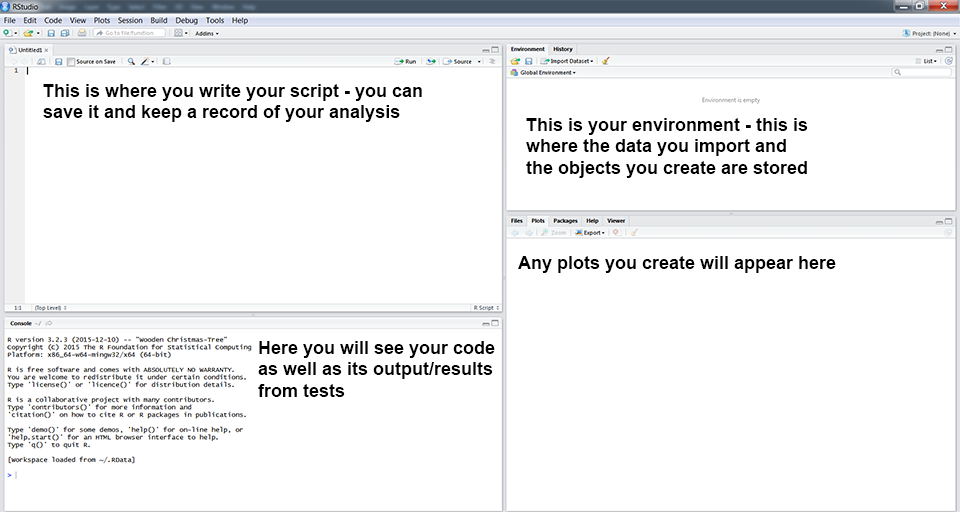
\includegraphics[width=1.1\textwidth]{figs/R_Studio.png}
	\caption{The RStudio Environment. Taken from OurCodingClub.io}
	\label{fig:R_Studio}
\end{figure} 

On the lower left is the \textit{Console} pane - this is the engine of R. You can give instructions to R by directly typing at the prompt (\code{>}). 
\\

On the upper left is your R Script - here, you can write commands and send them to the console by clicking ``\texttt{Run}'' or by typing \code{Ctrl-Enter} (or \code{Cmd-Enter}). Notice that all lines are preceded by \code{\#} - this is the comment character in R.
\\

On the lower right, you can browse the packages installed on your machine, open files and search R Help. This pane will also show plots when we run them later in the practical.
\\


\fbox{\begin{minipage}{36em}
\Large{\textbf{Exercise 1.}}

\normalsize
Try running some basic commands directly in the console and from the R Script:
\end{minipage}}


\begin{shaded}
\begin{Schunk}
\begin{Sinput}
> 2+3
> 1:10
> seq(1, 20, 4)
> mean(c(3, 6, 9, 3, 6, 7))
\end{Sinput}
\end{Schunk}
\end{shaded}

\fbox{\begin{minipage}{36em}
Let's assign a sequence of numbers to an object, \code{x}:
\end{minipage}}

\begin{shaded}
\begin{Schunk}
\begin{Sinput}
> x <- 1:10
> x
> y <- seq(0, 4.5, 0.5)
> y
\end{Sinput}
\end{Schunk}
\end{shaded}


You can see that in the upper right pane, we can see this new objects \code{x} and \code{y} in the environment.

\subsection {Finding Help within R.}

The fastest way to find help in R is to search using \code{?}. For example:

\begin{shaded}
\begin{Schunk}
\begin{Sinput}
> ?mean
\end{Sinput}
\end{Schunk}
\end{shaded}

should bring up a help page for the function \code{mean()} in the lower right corner. Typing two question marks: 

\begin{shaded}
\begin{Schunk}
\begin{Sinput}
> ??mean
> ??"standard error"
\end{Sinput}
\end{Schunk}
\end{shaded}

will search all help files and return a list of those that match. \\\\

\fbox{\begin{minipage}{36em}
\Large{\textbf{Exercise 2.}}

\normalsize
\begin{enumerate}
\item Using only \code{?} and/or \code{??}, find a function for calculating the standard deviation. What is the standard deviation of \code{x}?

\item Using \code{?}, find the help file for the \code{sort()} function. Sort \code{x} and \code{y} in reverse order.\\
\end{enumerate}
\end{minipage}}


\subsection {Troubleshooting and finding help outside of R.}

\begin{itemize}
\item Coding Club Tutorials \& Useful Links \url{https://ourcodingclub.github.io/}
\item Stack Overflow \url{https://stackoverflow.com/}: Try searching with the tag [R]
\item RStudio Cheatsheets \url{https://www.rstudio.com/resources/cheatsheets/}
\end{itemize}


%-------------------------------------------
\section {Loading and Preparing Data.}
%--------------------------------------------

Now that we are familiar with the RStusio environment, it's time to start working with real data. \\

In the folder \texttt{data}, you have been provided with a single dataset on Peruvian Soil in two common formats - \texttt{.txt} (tab-delimited) and \texttt{.csv} (comma-delimited). \\

The easiest way to read the data into R is to use the \texttt{Import dataset} button in the Environment tab, selecting \texttt{From Text (base)...} and choosing either datafile (\texttt{.txt} or \texttt{.csv}). A box will appear (Figure \ref{fig:Import_Dataset2}). Check each of the options that applies to the data (i.e. change nothing) and click ``\texttt{Import}''. You will notice that the object \texttt{Peru\_Soil\_Data} is now in the R environment, but you may also have noticed a command appearing in the Console: \\


\begin{figure}[t]
	\centering 
	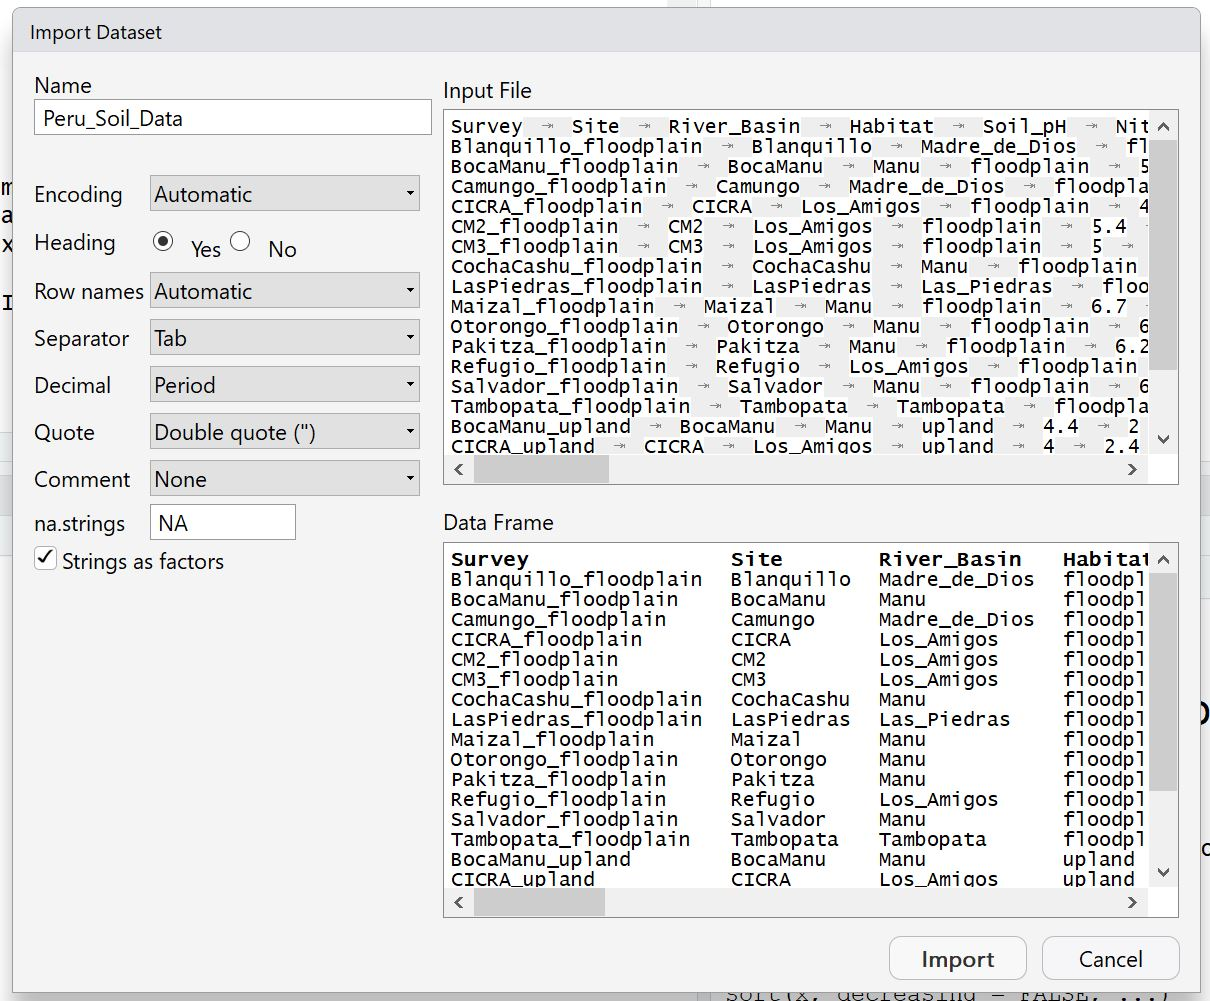
\includegraphics[width=0.8\textwidth]{figs/Import_Dataset2.JPG}
	\caption{Importing data manually into R}
	\label{fig:Import_Dataset2}
\end{figure} 



\begin{shaded}
\begin{Schunk}
\begin{Sinput}
> Peru_Soil_Data <- read.delim("C:/Users/sjohns10/Google Drive/
+ Teaching and Seminars/201711 NERC E3 DTP/Intro_to_R/data/
+ Peru_Soil_Data.txt")
\end{Sinput}
\end{Schunk}
\end{shaded}

This command can be copied and pasted into your script, which would save you from clicking the next time. However, providing such a long path if problematic - if you were to rename one of the directories, or move the folder somewhere else, then the code would no longer work. \\

RProjects provide the solution to this. Try typing the following into your script, and guiding the command to the data file using the \texttt{Tab} key:

\begin{shaded}
\texttt{Peru\_Soil\_Data <- read.delim("}
\end{shaded}

You should now have the following code in your script:

\begin{shaded}
\begin{Schunk}
\begin{Sinput}
> Peru_Soil_Data <- read.delim("data/Peru_Soil_Data.txt")
\end{Sinput}
\end{Schunk}
\end{shaded}




\end{document}
